% Created 2019-10-28 ma 14:56
% Intended LaTeX compiler: pdflatex
\documentclass[12pt]{article}

%%%% settings when exporting code %%%% 

\usepackage{listings}
\lstset{
backgroundcolor=\color{white},
basewidth={0.5em,0.4em},
basicstyle=\ttfamily\small,
breakatwhitespace=false,
breaklines=true,
columns=fullflexible,
commentstyle=\color[rgb]{0.5,0,0.5},
frame=single,
keepspaces=true,
keywordstyle=\color{black},
literate={~}{$\sim$}{1},
numbers=left,
numbersep=10pt,
numberstyle=\ttfamily\tiny\color{gray},
showspaces=false,
showstringspaces=false,
stepnumber=1,
stringstyle=\color[rgb]{0,.5,0},
tabsize=4,
xleftmargin=.23in,
emph={anova,apply,class,coef,colnames,colNames,colSums,dim,dcast,for,ggplot,head,if,ifelse,is.na,lapply,list.files,library,logLik,melt,plot,require,rowSums,sapply,setcolorder,setkey,str,summary,tapply},
emphstyle=\color{blue}
}

%%%% packages %%%%%

\usepackage[utf8]{inputenc}
\usepackage[T1]{fontenc}
\usepackage{lmodern}
\usepackage{textcomp}
\usepackage{color}
\usepackage{enumerate}
\usepackage{graphicx}
\usepackage{grffile}
\usepackage{wrapfig}
\usepackage{rotating}
\usepackage{longtable}
\usepackage{multirow}
\usepackage{multicol}
\usepackage{changes}
\usepackage{pdflscape}
\usepackage{geometry}
\usepackage[normalem]{ulem}
\usepackage{amssymb}
\usepackage{amsmath}
\usepackage{amsfonts}
\usepackage{dsfont}
\usepackage{array}
\usepackage{ifthen}
\usepackage{hyperref}
\usepackage{natbib}
%
%%%% specifications %%%%
%
\usepackage{ifthen}
\usepackage{xifthen}
\usepackage{xargs}
\usepackage{xspace}
\newcommand\Rlogo{\textbf{\textsf{R}}\xspace} %
\RequirePackage{fancyvrb}
\DefineVerbatimEnvironment{verbatim}{Verbatim}{fontsize=\small,formatcom = {\color[rgb]{0.5,0,0}}}
\RequirePackage{colortbl} % arrayrulecolor to mix colors
\RequirePackage{setspace} % to modify the space between lines - incompatible with footnote in beamer
\renewcommand{\baselinestretch}{1.1}
\geometry{top=1cm}
\RequirePackage{epstopdf} % to be able to convert .eps to .pdf image files
\RequirePackage{capt-of} %
\RequirePackage{caption} % newlines in graphics
\RequirePackage{amsmath}
\RequirePackage{algorithm}
\RequirePackage[noend]{algpseudocode}
\RequirePackage{dsfont}
\RequirePackage{amsmath,stmaryrd,graphicx}
\RequirePackage{prodint} % product integral symbol (\PRODI)
\newcommand\defOperator[7]{%
\ifthenelse{\isempty{#2}}{
\ifthenelse{\isempty{#1}}{#7{#3}#4}{#7{#3}#4 \left#5 #1 \right#6}
}{
\ifthenelse{\isempty{#1}}{#7{#3}#4_{#2}}{#7{#3}#4_{#1}\left#5 #2 \right#6}
}
}
\newcommand\defUOperator[5]{%
\ifthenelse{\isempty{#1}}{
#5\left#3 #2 \right#4
}{
\ifthenelse{\isempty{#2}}{\underset{#1}{\operatornamewithlimits{#5}}}{
\underset{#1}{\operatornamewithlimits{#5}}\left#3 #2 \right#4}
}
}
\newcommand{\defBoldVar}[2]{
\ifthenelse{\equal{#2}{T}}{\boldsymbol{#1}}{\mathbf{#1}}
}
\newcommandx\Cov[2][1=,2=]{\defOperator{#1}{#2}{C}{ov}{\lbrack}{\rbrack}{\mathbb}}
\newcommandx\Esp[2][1=,2=]{\defOperator{#1}{#2}{E}{}{\lbrack}{\rbrack}{\mathbb}}
\newcommandx\Prob[2][1=,2=]{\defOperator{#1}{#2}{P}{}{\lbrack}{\rbrack}{\mathbb}}
\newcommandx\Qrob[2][1=,2=]{\defOperator{#1}{#2}{Q}{}{\lbrack}{\rbrack}{\mathbb}}
\newcommandx\Var[2][1=,2=]{\defOperator{#1}{#2}{V}{ar}{\lbrack}{\rbrack}{\mathbb}}
\newcommandx\Binom[2][1=,2=]{\defOperator{#1}{#2}{B}{}{(}{)}{\mathcal}}
\newcommandx\Gaus[2][1=,2=]{\defOperator{#1}{#2}{N}{}{(}{)}{\mathcal}}
\newcommandx\Wishart[2][1=,2=]{\defOperator{#1}{#2}{W}{ishart}{(}{)}{\mathcal}}
\newcommandx\Likelihood[2][1=,2=]{\defOperator{#1}{#2}{L}{}{(}{)}{\mathcal}}
\newcommandx\Information[2][1=,2=]{\defOperator{#1}{#2}{I}{}{(}{)}{\mathcal}}
\newcommandx\Score[2][1=,2=]{\defOperator{#1}{#2}{S}{}{(}{)}{\mathcal}}
\newcommandx\Vois[2][1=,2=]{\defOperator{#1}{#2}{V}{}{(}{)}{\mathcal}}
\newcommandx\IF[2][1=,2=]{\defOperator{#1}{#2}{IF}{}{(}{)}{\mathcal}}
\newcommandx\Ind[1][1=]{\defOperator{}{#1}{1}{}{(}{)}{\mathds}}
\newcommandx\Max[2][1=,2=]{\defUOperator{#1}{#2}{(}{)}{min}}
\newcommandx\Min[2][1=,2=]{\defUOperator{#1}{#2}{(}{)}{max}}
\newcommandx\argMax[2][1=,2=]{\defUOperator{#1}{#2}{(}{)}{argmax}}
\newcommandx\argMin[2][1=,2=]{\defUOperator{#1}{#2}{(}{)}{argmin}}
\newcommandx\cvD[2][1=D,2=n \rightarrow \infty]{\xrightarrow[#2]{#1}}
\newcommandx\Hypothesis[2][1=,2=]{
\ifthenelse{\isempty{#1}}{
\mathcal{H}
}{
\ifthenelse{\isempty{#2}}{
\mathcal{H}_{#1}
}{
\mathcal{H}^{(#2)}_{#1}
}
}
}
\newcommandx\dpartial[4][1=,2=,3=,4=\partial]{
\ifthenelse{\isempty{#3}}{
\frac{#4 #1}{#4 #2}
}{
\left.\frac{#4 #1}{#4 #2}\right\rvert_{#3}
}
}
\newcommandx\dTpartial[3][1=,2=,3=]{\dpartial[#1][#2][#3][d]}
\newcommandx\ddpartial[3][1=,2=,3=]{
\ifthenelse{\isempty{#3}}{
\frac{\partial^{2} #1}{\left( \partial #2\right)^2}
}{
\frac{\partial^2 #1}{\partial #2\partial #3}
}
}
\newcommand\Real{\mathbb{R}}
\newcommand\Rational{\mathbb{Q}}
\newcommand\Natural{\mathbb{N}}
\newcommand\trans[1]{{#1}^\intercal}%\newcommand\trans[1]{{\vphantom{#1}}^\top{#1}}
\newcommand{\independent}{\mathrel{\text{\scalebox{1.5}{$\perp\mkern-10mu\perp$}}}}
\newcommand\half{\frac{1}{2}}
\newcommand\normMax[1]{\left|\left|#1\right|\right|_{max}}
\newcommand\normTwo[1]{\left|\left|#1\right|\right|_{2}}
\author{Brice Ozenne}
\date{\today}
\title{A simple example of multiple imputation using the mice package}
\hypersetup{
 colorlinks=true,
 citecolor=[rgb]{0,0.5,0},
 urlcolor=[rgb]{0,0,0.5},
 linkcolor=[rgb]{0,0,0.5},
 pdfauthor={Brice Ozenne},
 pdftitle={A simple example of multiple imputation using the mice package},
 pdfkeywords={},
 pdfsubject={},
 pdfcreator={Emacs 25.2.1 (Org mode 9.0.4)},
 pdflang={English}
 }
\begin{document}

\maketitle
This document gathers code from the documentation of the mice
package. See \url{https://stefvanbuuren.name/mice/}.

\bigskip

Load packages
\lstset{language=r,label= ,caption= ,captionpos=b,numbers=none}
\begin{lstlisting}
library(lava)
library(mice)
library(data.table)
library(ggplot2)
\end{lstlisting}

\section{Simulate data (just to have an example to work with)}
\label{sec:org1461e79}
Generative model
\lstset{language=r,label= ,caption= ,captionpos=b,numbers=none}
\begin{lstlisting}
mSim <- lvm(Y~group+season+bmi+gender+age)
categorical(mSim, labels = c("winter","summer")) <- ~season
categorical(mSim, labels = c("SAD","HC")) <- ~group
categorical(mSim, labels = c("Male","Female")) <- ~gender
distribution(mSim,~bmi) <- lava::gaussian.lvm(mean = 22, sd = 3)
distribution(mSim,~age) <- lava::uniform.lvm(20,80)
\end{lstlisting}

Sampling
\lstset{language=r,label= ,caption= ,captionpos=b,numbers=none}
\begin{lstlisting}
n <- 1e2
set.seed(10)
dt.data <- as.data.table(sim(mSim,n))
\end{lstlisting}

Add missing values
\lstset{language=r,label= ,caption= ,captionpos=b,numbers=none}
\begin{lstlisting}
dt.data[1:10, bmi:=NA]
\end{lstlisting}

\clearpage

\section{Working with mice}
\label{sec:org840cc6d}

\subsection{Step 1: Inspect the missing data pattern}
\label{sec:org6fd44ff}
Check the number of missing values in the dataset:
\lstset{language=r,label= ,caption= ,captionpos=b,numbers=none}
\begin{lstlisting}
colSums(is.na(dt.data))
\end{lstlisting}

\begin{verbatim}
Y  group season    bmi gender    age 
0      0      0     10      0      0
\end{verbatim}

Missing data patterns:   
\lstset{language=r,label= ,caption= ,captionpos=b,numbers=none}
\begin{lstlisting}
md.pattern(dt.data)
\end{lstlisting}

\begin{verbatim}
   Y group season gender age bmi   
90 1     1      1      1   1   1  0
10 1     1      1      1   1   0  1
   0     0      0      0   0  10 10
\end{verbatim}

\begin{center}
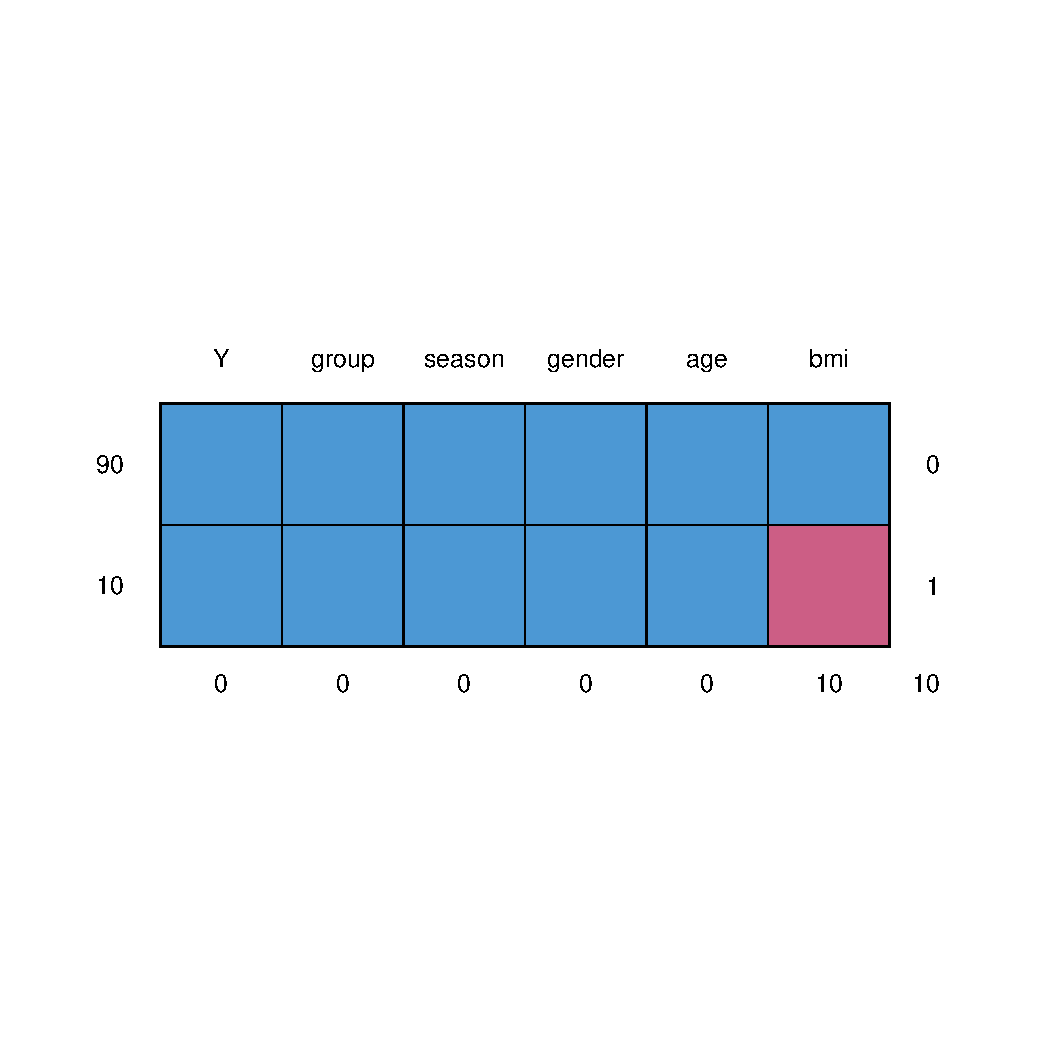
\includegraphics[width=.9\linewidth]{./missingDataPattern.pdf}
\end{center}

\clearpage

\subsection{Step 2: Define imputation model}
\label{sec:orgeaf40b3}

\lstset{language=r,label= ,caption= ,captionpos=b,numbers=none}
\begin{lstlisting}
all.variables <- c("Y","group","season","bmi","gender","age")
n.variables <- length(all.variables)
Mlink <- matrix(0, n.variables, n.variables,
				dimnames = list(all.variables,all.variables))
Mlink["bmi",c("group","season","gender","age")] <- 1
Mlink
\end{lstlisting}

\begin{verbatim}
       Y group season bmi gender age
Y      0     0      0   0      0   0
group  0     0      0   0      0   0
season 0     0      0   0      0   0
bmi    0     1      1   0      1   1
gender 0     0      0   0      0   0
age    0     0      0   0      0   0
\end{verbatim}

A value of 1 means that the column variable is used as a predictor for
 the target block (in the rows).

\clearpage

\subsection{Step 3: Generate imputed datasets}
\label{sec:org0287794}
Generate imputed values
\lstset{language=r,label= ,caption= ,captionpos=b,numbers=none}
\begin{lstlisting}
n.imputed <- 3 ## number of imputed datasets
dt.mice <- mice(dt.data,
				m=n.imputed, 
				maxit = 50, # number of iterations to obtain the imputed dataset
				predictorMatrix = Mlink,
				method = 'pmm', # Predictive mean matching, only ok for continuous variables, it is possible to set constrains for positive variables
				seed = 500, printFlag = FALSE)
summary(dt.mice)
\end{lstlisting}

\begin{verbatim}
Class: mids
Number of multiple imputations:  3 
Imputation methods:
     Y  group season    bmi gender    age 
    ""     ""     ""  "pmm"     ""     "" 
PredictorMatrix:
       Y group season bmi gender age
Y      0     0      0   0      0   0
group  0     0      0   0      0   0
season 0     0      0   0      0   0
bmi    0     1      1   0      1   1
gender 0     0      0   0      0   0
age    0     0      0   0      0   0
\end{verbatim}

\clearpage

\subsection{Step 4: Check the imputed datasets}
\label{sec:org3513128}
\subsubsection{Convergence of the imputation algorithm}
\label{sec:orga0ec3c8}

\lstset{language=r,label= ,caption= ,captionpos=b,numbers=none}
\begin{lstlisting}
plot(dt.mice)
\end{lstlisting}

\begin{center}
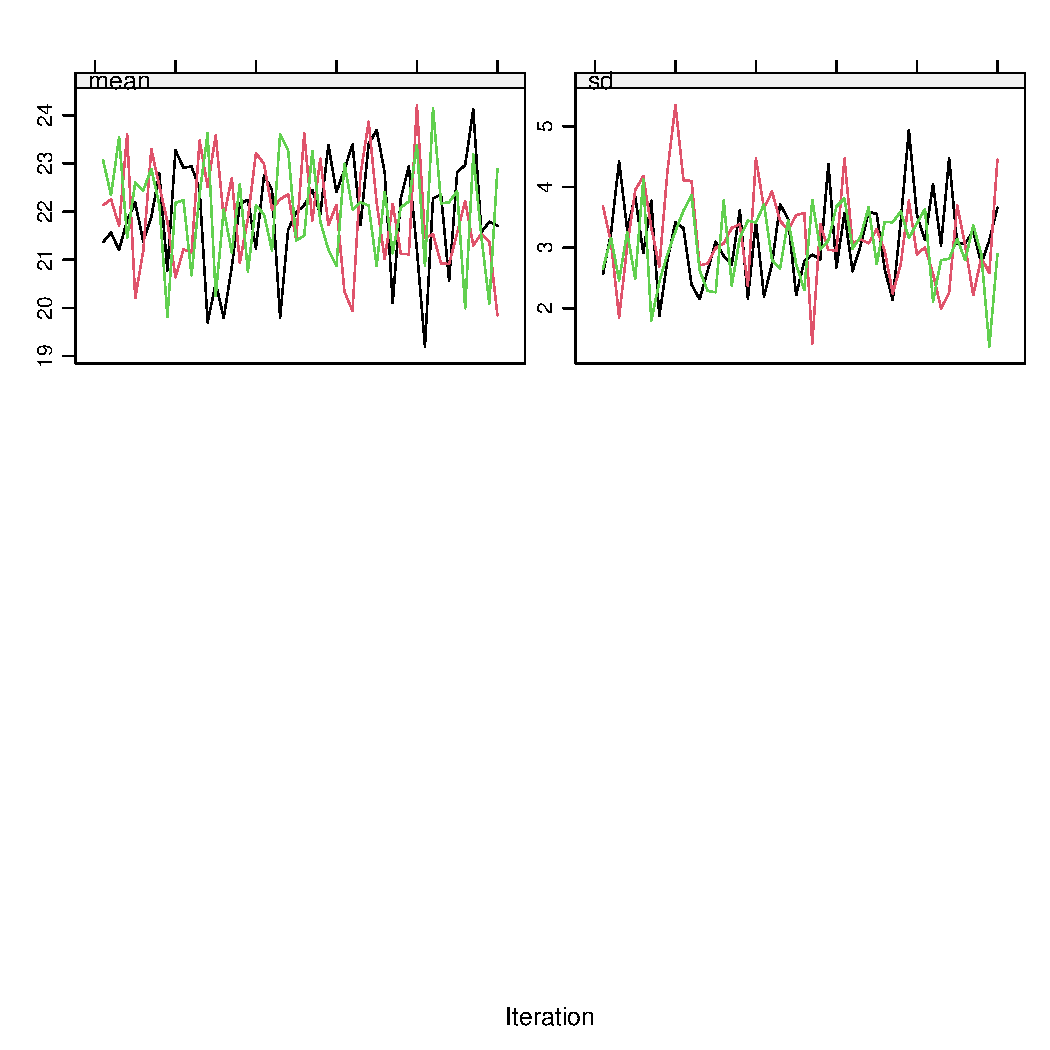
\includegraphics[width=.9\linewidth]{./traceCVimputed.pdf}
\end{center}

\subsubsection{Visualizing the imputed values}
\label{sec:org569670e}
Visualize imputed value values and check they are plausible (e.g. mice
is not imputed a BMI of 75):
\lstset{language=r,label= ,caption= ,captionpos=b,numbers=none}
\begin{lstlisting}
dt.mice$imp$bmi
\end{lstlisting}

\begin{verbatim}
          1        2        3
1  25.68855 25.31909 21.60139
2  27.25524 15.38820 19.28934
3  25.31909 22.82264 21.60139
4  21.94247 25.98147 24.80171
5  17.42985 21.94247 25.68855
6  22.68303 18.98739 20.97076
7  21.82216 21.93016 22.82264
8  19.81314 21.13770 26.03528
9  22.82264 21.88207 25.68855
10 19.87741 18.29777 22.31832
\end{verbatim}

The rows correspond to the 3 different imputed datasets and the
columns to 10 imputed values per dataset. One can also summarizes the
imputed values computing their quantiles:

\lstset{language=r,label= ,caption= ,captionpos=b,numbers=none}
\begin{lstlisting}
apply(dt.mice$imp$bmi,2,quantile)
\end{lstlisting}

\begin{verbatim}
            1        2        3
0%   17.42985 15.38820 19.28934
25%  20.36360 19.52497 21.60139
50%  22.31275 21.90611 22.57048
75%  24.69498 22.60260 25.46684
100% 27.25524 25.98147 26.03528
\end{verbatim}

Boxplot of the imputed values:

\lstset{language=r,label= ,caption= ,captionpos=b,numbers=none}
\begin{lstlisting}
boxplot(dt.mice$imp$bmi)
\end{lstlisting}

\begin{center}
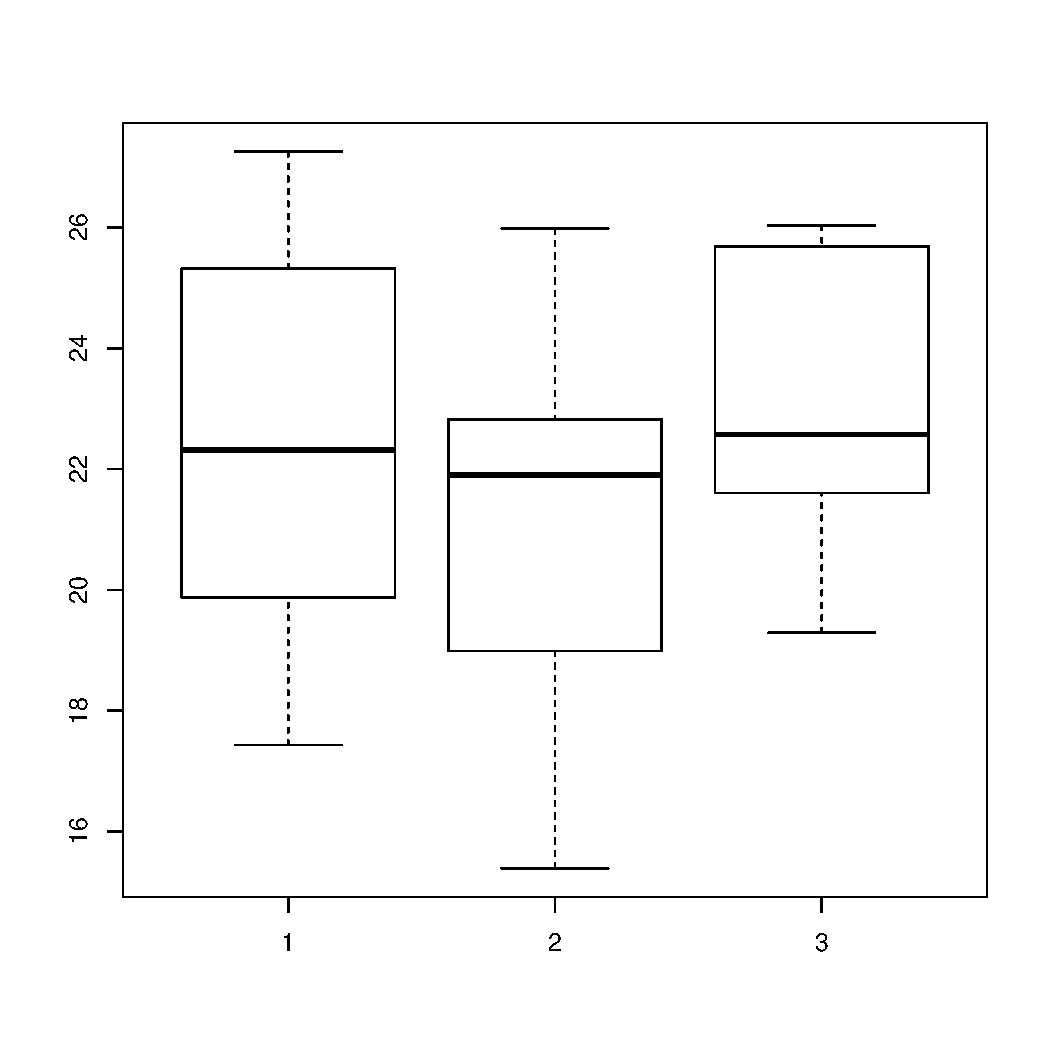
\includegraphics[width=.9\linewidth]{./boxplotImputed.pdf}
\end{center}

Imputed values vs. observed values
\lstset{language=r,label= ,caption= ,captionpos=b,numbers=none}
\begin{lstlisting}
dt.bmi <- rbind(data.table(bmi = unlist(dt.mice$imp$bmi), imputed = TRUE),
				data.table(bmi = na.omit(dt.data$bmi), imputed = FALSE))
\end{lstlisting}

Histogram
\lstset{language=r,label= ,caption= ,captionpos=b,numbers=none}
\begin{lstlisting}
gg1.bmi <- ggplot(dt.bmi, aes(bmi, group = imputed, fill = imputed))
gg1.bmi <- gg1.bmi + geom_histogram(aes(y=..count../sum(..count..)),position = "dodge")
gg1.bmi
\end{lstlisting}

\begin{verbatim}
`stat_bin()` using `bins = 30`. Pick better value with `binwidth`.
\end{verbatim}

\begin{center}
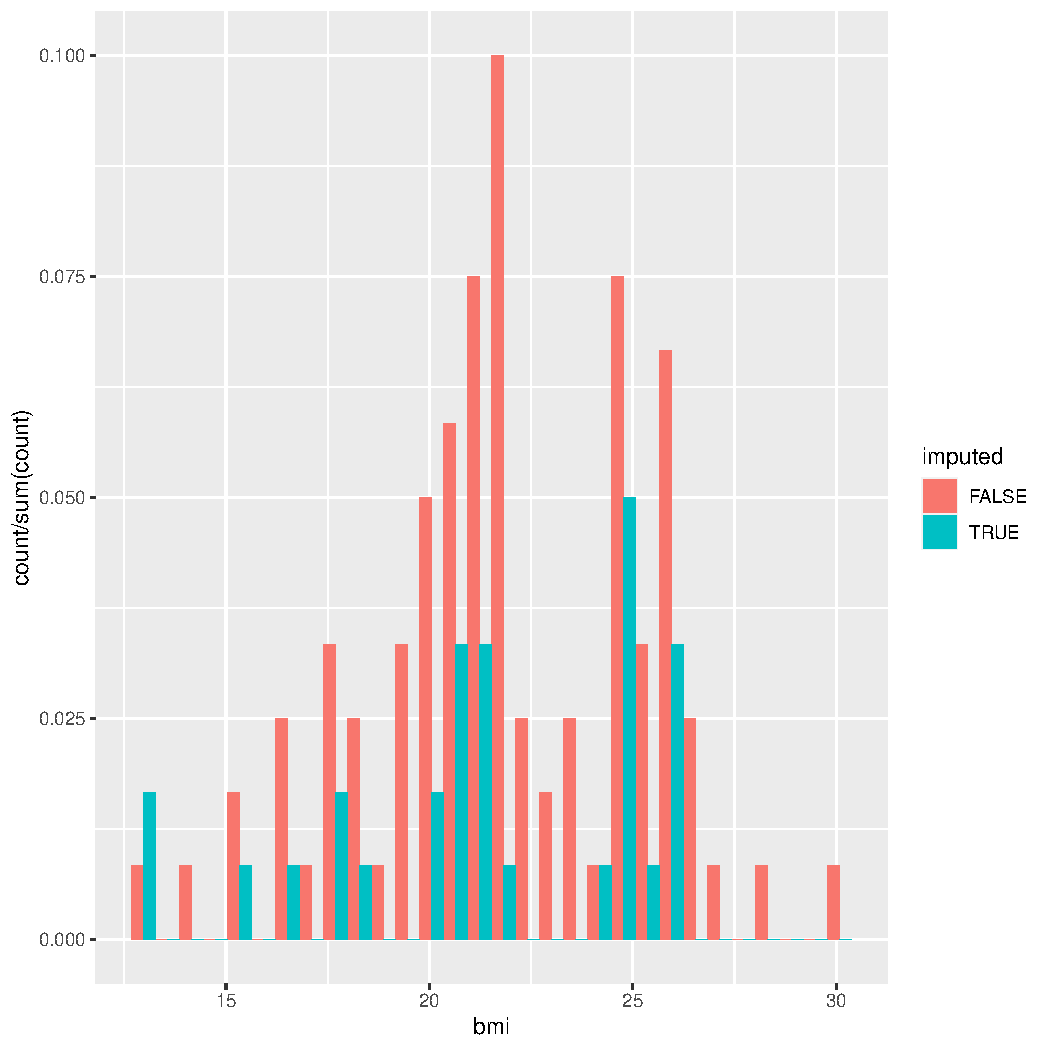
\includegraphics[width=.9\linewidth]{./histImputed.pdf}
\end{center}

One more plot:

\lstset{language=r,label= ,caption= ,captionpos=b,numbers=none}
\begin{lstlisting}
stripplot(dt.mice, bmi~.imp, pch=20, cex=2)
\end{lstlisting}

\begin{center}
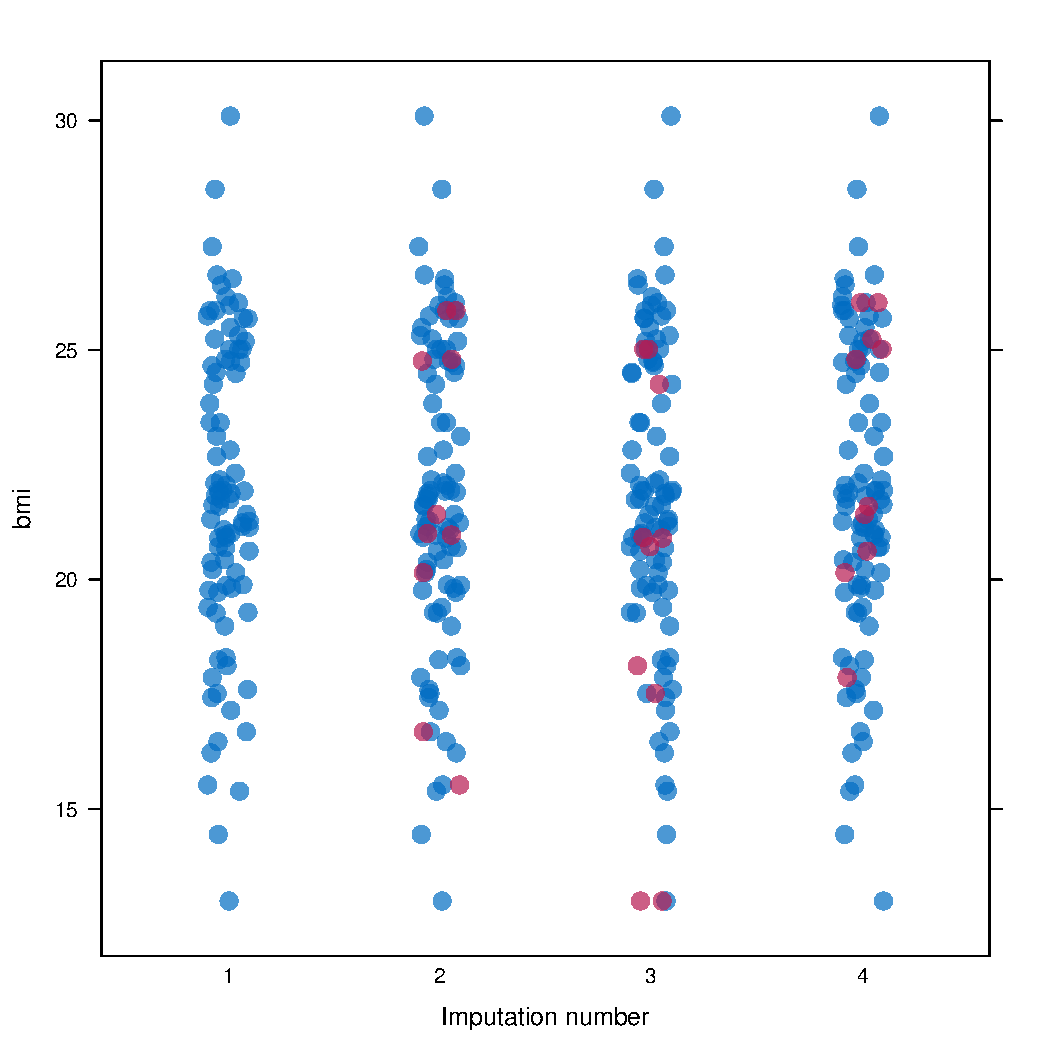
\includegraphics[width=.9\linewidth]{./striplotImputed.pdf}
\end{center}

\clearpage

\subsection{Step 3: Fit the statical model on each imputed dataset}
\label{sec:orge0e1b9a}

\lstset{language=r,label= ,caption= ,captionpos=b,numbers=none}
\begin{lstlisting}
e.mice <- with(data = dt.mice,
			   lm(Y~group+season+bmi+gender+age)
			   )
e.mice
\end{lstlisting}

\begin{verbatim}
call :
with.mids(data = dt.mice, expr = lm(Y ~ group + season + bmi + 
    gender + age))

call1 :
mice(data = dt.data, m = n.imputed, method = "pmm", predictorMatrix = Mlink, 
    maxit = 50, printFlag = FALSE, seed = 500)

nmis :
     Y  group season    bmi gender    age 
     0      0      0     10      0      0 

analyses :
[[1]]

Call:
lm(formula = Y ~ group + season + bmi + gender + age)

Coefficients:
 (Intercept)       groupHC  seasonsummer           bmi  genderFemale           age  
      0.5208        0.5992        0.7517        0.9735        0.7954        1.0058  


[[2]]

Call:
lm(formula = Y ~ group + season + bmi + gender + age)

Coefficients:
 (Intercept)       groupHC  seasonsummer           bmi  genderFemale           age  
      1.2661        0.8914        1.1338        0.9197        0.8447        1.0088  


[[3]]

Call:
lm(formula = Y ~ group + season + bmi + gender + age)

Coefficients:
 (Intercept)       groupHC  seasonsummer           bmi  genderFemale           age  
      1.1214        0.7458        1.4506        0.9159        0.8573        1.0081
\end{verbatim}

Check that using \texttt{with}:
\lstset{language=r,label= ,caption= ,captionpos=b,numbers=none}
\begin{lstlisting}
e.mice$analyses[[1]]
\end{lstlisting}

\begin{verbatim}

Call:
lm(formula = Y ~ group + season + bmi + gender + age)

Coefficients:
 (Intercept)       groupHC  seasonsummer           bmi  genderFemale           age  
      0.5208        0.5992        0.7517        0.9735        0.7954        1.0058
\end{verbatim}

is equivalent to run the linear regression on the imputed dataset:
\lstset{language=r,label= ,caption= ,captionpos=b,numbers=none}
\begin{lstlisting}
dt.tempo <- copy(dt.data)
dt.tempo[is.na(bmi), bmi := dt.mice$imp$bmi[,1]]
lm(Y ~ group + season + bmi + gender + age, data  = dt.tempo)
\end{lstlisting}

\begin{verbatim}

Call:
lm(formula = Y ~ group + season + bmi + gender + age, data = dt.tempo)

Coefficients:
 (Intercept)       groupHC  seasonsummer           bmi  genderFemale           age  
      0.5208        0.5992        0.7517        0.9735        0.7954        1.0058
\end{verbatim}

\clearpage

\subsection{Step 4: Pool the results over the imputed datasets}
\label{sec:org22b16ae}

\lstset{language=r,label= ,caption= ,captionpos=b,numbers=none}
\begin{lstlisting}
ePool.mice <- pool(e.mice)
summary(ePool.mice)
\end{lstlisting}

\begin{verbatim}
              estimate   std.error  statistic        df    p.value
(Intercept)  0.9694266 1.332790683   0.727366 52.148057 0.46888374
groupHC      0.7454997 0.379770099   1.963029 30.298012 0.05272075
seasonsummer 1.1120467 0.527089351   2.109788  5.024377 0.03764349
bmi          0.9363468 0.063722009  14.694245 13.428456 0.00000000
genderFemale 0.8324731 0.338852458   2.456742 90.285942 0.01593243
age          1.0075630 0.009578818 105.186567 84.307182 0.00000000
\end{verbatim}


The (pooled) estimate is the average of the estimates relative to each
imputed dataset:
\lstset{language=r,label= ,caption= ,captionpos=b,numbers=none}
\begin{lstlisting}
Q.coef <- colMeans(do.call(rbind,lapply(e.mice$analyses, coef)))
Q.coef
\end{lstlisting}

\begin{verbatim}
(Intercept)      groupHC seasonsummer          bmi genderFemale          age 
  0.9694266    0.7454997    1.1120467    0.9363468    0.8324731    1.0075630
\end{verbatim}

The variance is a bit more complex and involves:
\begin{itemize}
\item the within-imputation variance (depends on the sample size)
\end{itemize}
\lstset{language=r,label= ,caption= ,captionpos=b,numbers=none}
\begin{lstlisting}
covW <- Reduce("+",lapply(e.mice$analyses, vcov))/n.imputed
covW
\end{lstlisting}

\begin{verbatim}
              (Intercept)      groupHC  seasonsummer           bmi  genderFemale           age
(Intercept)   1.568091910 -0.093480148 -0.0399097160 -5.728182e-02 -0.0843633775 -3.366141e-03
groupHC      -0.093480148  0.115763163  0.0094967612  2.269357e-03  0.0048518076 -4.621780e-04
seasonsummer -0.039909716  0.009496761  0.1145514144 -1.233739e-03  0.0103324967 -1.316344e-04
bmi          -0.057281821  0.002269357 -0.0012337388  2.677583e-03  0.0001937303 -3.977686e-05
genderFemale -0.084363377  0.004851808  0.0103324967  1.937303e-04  0.1133952760  1.912624e-04
age          -0.003366141 -0.000462178 -0.0001316344 -3.977686e-05  0.0001912624  8.855684e-05
\end{verbatim}

\begin{itemize}
\item the between-imputation variance (depends on the amount of missing data)
\end{itemize}
\lstset{language=r,label= ,caption= ,captionpos=b,numbers=none}
\begin{lstlisting}
ls.diffCoef <- lapply(e.mice$analyses, function(iI){coef(iI)-Q.coef})
covB <- Reduce("+",lapply(ls.diffCoef,tcrossprod))/(n.imputed-1)
covB
\end{lstlisting}

\begin{verbatim}
             [,1]         [,2]          [,3]          [,4]          [,5]          [,6]
[1,]  0.156179320  0.054483744  0.1097704140 -1.235176e-02  0.0120121980  6.112650e-04
[2,]  0.054483744  0.021346623  0.0279984041 -3.933280e-03  0.0036072493  2.167560e-04
[3,]  0.109770414  0.027998404  0.1224538273 -1.033447e-02  0.0110091756  4.141649e-04
[4,] -0.012351758 -0.003933280 -0.0103344679  1.037183e-03 -0.0010436570 -4.777893e-05
[5,]  0.012012198  0.003607249  0.0110091756 -1.043657e-03  0.0010692841  4.613820e-05
[6,]  0.000611265  0.000216756  0.0004141649 -4.777893e-05  0.0000461382  2.397687e-06
\end{verbatim}

\begin{itemize}
\item the simulation error
\end{itemize}
\lstset{language=r,label= ,caption= ,captionpos=b,numbers=none}
\begin{lstlisting}
covE <- covB/n.imputed
covE
\end{lstlisting}

\begin{verbatim}
             [,1]         [,2]         [,3]          [,4]          [,5]          [,6]
[1,]  0.052059773  0.018161248  0.036590138 -4.117253e-03  0.0040040660  2.037550e-04
[2,]  0.018161248  0.007115541  0.009332801 -1.311093e-03  0.0012024164  7.225200e-05
[3,]  0.036590138  0.009332801  0.040817942 -3.444823e-03  0.0036697252  1.380550e-04
[4,] -0.004117253 -0.001311093 -0.003444823  3.457278e-04 -0.0003478857 -1.592631e-05
[5,]  0.004004066  0.001202416  0.003669725 -3.478857e-04  0.0003564280  1.537940e-05
[6,]  0.000203755  0.000072252  0.000138055 -1.592631e-05  0.0000153794  7.992289e-07
\end{verbatim}

The total variance is:
\lstset{language=r,label= ,caption= ,captionpos=b,numbers=none}
\begin{lstlisting}
covT <- covW + covB + covE
\end{lstlisting}

leading to the standard errors:
\lstset{language=r,label= ,caption= ,captionpos=b,numbers=none}
\begin{lstlisting}
sqrt(diag(covT))
\end{lstlisting}
\begin{verbatim}
(Intercept)      groupHC seasonsummer          bmi genderFemale          age 
1.332790683  0.379770099  0.527089351  0.063722009  0.338852458  0.009578818
\end{verbatim}

\clearpage

\section{Special case: imputation using a specific law and no covariate}
\label{sec:orgde8e1b1}
Mice can be adapted in order, for instance, to sample from a uniform
distribution or a truncated normal distribution. First define a
function able to generate data like:
\lstset{language=r,label= ,caption= ,captionpos=b,numbers=none}
\begin{lstlisting}
mice.impute.SI_unif <- function(y, ry, ...){ ## truncated normal law
	require(truncnorm)
	n.NA <- sum(ry==FALSE)
	sample <- runif(n.NA, min = 0, max = 1)
	return(cbind(sample))
}
\end{lstlisting}

or

\lstset{language=r,label= ,caption= ,captionpos=b,numbers=none}
\begin{lstlisting}
mice.impute.SI_tnorm <- function(y, ry, ...){ ## truncated normal law
	require(truncnorm)
	n.NA <- sum(ry==FALSE)
	sample <- rtruncnorm(n.NA, a = 0, b = 1, mean = 1, sd = 0.1)
	return(cbind(sample))
}
\end{lstlisting}
Then prepare the matrix indicating which variable should be used
during the imputation:
\lstset{language=r,label= ,caption= ,captionpos=b,numbers=none}
\begin{lstlisting}
impute.var <- c("bmi","group")
Mlink2 <- matrix(0, 
				 nrow = length(impute.var), 
				 ncol = length(impute.var), 
				 dimnames = list(impute.var,impute.var))
Mlink2["bmi","group"] <- 1
Mlink2
\end{lstlisting}

\begin{verbatim}
      bmi group
bmi     0     1
group   0     0
\end{verbatim}

\clearpage 

Then run mice as usual except that the method should correspond to one of the previous functions:
\lstset{language=r,label= ,caption= ,captionpos=b,numbers=none}
\begin{lstlisting}
n.imputed <- 50 ## number of imputed datasets
set.seed(1)
dt.mice2 <- mice(dt.data,
				 m=n.imputed, 
				 maxit = 1, # not relevant
				 predictorMatrix = Mlink2, # not relevant
				 method = 'SI_tnorm', # function previous define (without "mice.impute.")
				 seed = 500, printFlag = FALSE)
\end{lstlisting}

Then as usual one should check that the imputed values are satisfying:
\lstset{language=r,label= ,caption= ,captionpos=b,numbers=none}
\begin{lstlisting}
quantile(unlist(dt.mice2$imp$bmi))
\end{lstlisting}

\begin{verbatim}
       0%       25%       50%       75%      100% 
0.7041556 0.8790477 0.9317021 0.9687630 0.9997288
\end{verbatim}


\lstset{language=r,label= ,caption= ,captionpos=b,numbers=none}
\begin{lstlisting}
hist(unlist(dt.mice2$imp$bmi))
\end{lstlisting}

\begin{center}
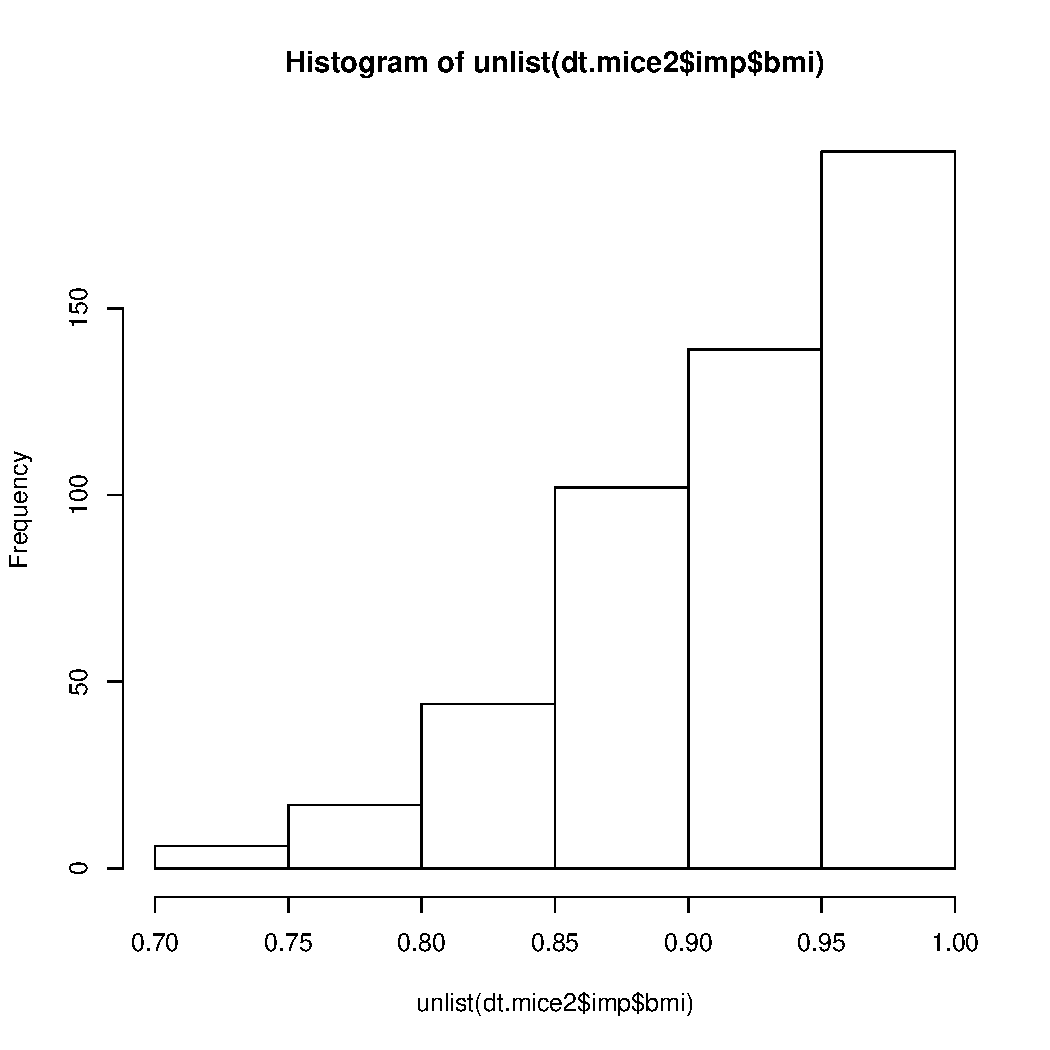
\includegraphics[width=.9\linewidth]{./histImputed2.pdf}
\end{center}

\clearpage

One more plot:
\lstset{language=r,label= ,caption= ,captionpos=b,numbers=none}
\begin{lstlisting}
stripplot(dt.mice2, bmi~.imp, pch=20, cex=2)
\end{lstlisting}

\begin{center}
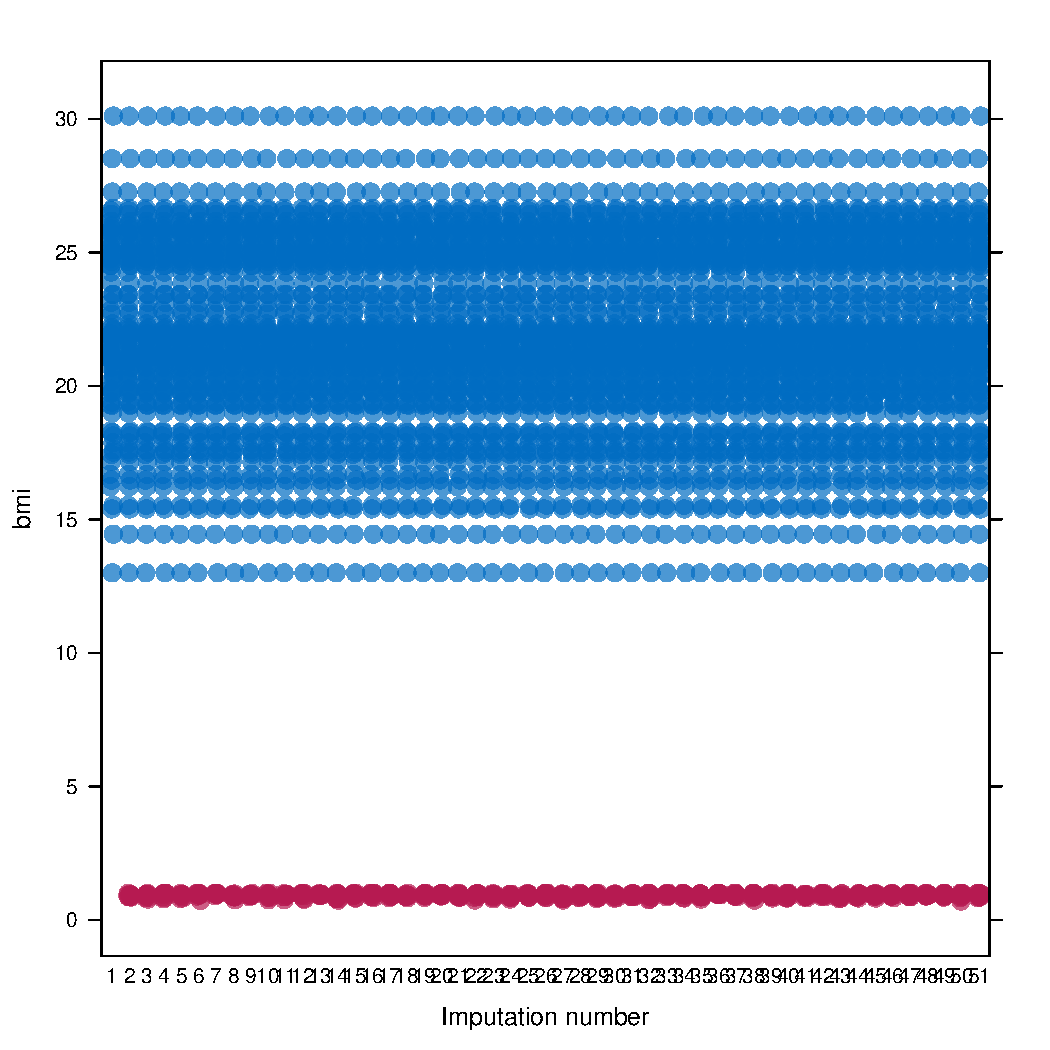
\includegraphics[width=.9\linewidth]{./striplotImputed2.pdf}
\end{center}

Here for instance the imputed values does not overlap the observed one
so something (i.e. the parameters of the distribution used for the
imputation) is wrong.

\section{Reporting guideline}
\label{sec:org45fe490}
From \url{https://stefvanbuuren.name/Winnipeg/Lectures/Winnipeg.pdf}:
\begin{itemize}
\item Amount of missing data
\item Reasons for missingness
\item Differences between complete and incomplete data
\item Method used to account for missing data
\item Software
\item Number of imputed datasets
\item Imputation model
\item Derived variables
\item Diagnostics
\item Pooling
\item Listwise deletion
\item Sensitivity analysis
\end{itemize}
\end{document}